\documentclass{article}

\newcommand{\ep}{\rule{.06in}{.1in}}
\textheight 9.5in

\usepackage{amssymb, bm}
\usepackage{amsmath}
\usepackage{amsthm}
\usepackage{graphicx, subcaption, booktabs}
\graphicspath{{/Users/andrewwork/thesis/jump-velocity/plots/}}

\usepackage{tikz, pgfplots, pgfplotstable, chemfig, xcolor}

% \usepgfplotslibrary{colorbrewer, statistics}
% \pgfplotsset{
%   exact axis/.style={grid=major, minor tick num=4, xlabel=$v^*$,
%     legend entries={PDF, CDF},},
%   every axis plot post/.append style={thick},
%   table/search
%   path={/Users/andrewwork/thesis/jump-velocity/dat-files},
%   colormap/YlGnBu,
%   cycle list/Set1-5,
%   legend style={legend cell align=left,},
% }

% \usepgfplotslibrary{external}
% \tikzexternalize

\renewcommand{\arraystretch}{1.2}
\pagestyle{empty} 
\oddsidemargin -0.25in
\evensidemargin -0.25in 
\topmargin -0.75in 
\parindent 0pt
\parskip 12pt
\textwidth 7in
%\font\cj=msbm10 at 12pt

\newcommand{\tn}{\textnormal}
\newcommand{\stiff}{\frac{k_f}{\gamma}}
\newcommand{\dd}{d}
\newcommand{\Der}[2]{\frac{\dd #1}{\dd #2}}
\newcommand{\Pder}[2]{\frac{\partial #1}{\partial #2}}
\newcommand{\Integral}[4]{\int_{#3}^{#4} {#1} \dd #2}
\newcommand{\vect}[1]{\boldsymbol{\mathbf{#1}}}
\newcommand{\mat}[1]{\underline{\underline{#1}}}
\DeclareMathOperator{\Exp}{Exp}

% Text width is 7 inches

\def\R{\mathbb{R}}
\def\N{\mathbb{N}}
\def\C{\mathbb{C}}
\def\Z{\mathbb{Z}}
\def\Q{\mathbb{Q}}
\def\H{\mathbb{H}}
\def\B{\mathcal{B}} 
%\topmargin -.5in 

\setcounter{secnumdepth}{2}
\begin{document}
\pagestyle{plain}

\begin{center}
  {\Large Meeting Notes (\today)}
\end{center}

{\large \textbf{Follow-up from last week}}

\begin{itemize}
\item Check $\displaystyle{\Der{\|\vect{e}_m\|}{t} \equiv 0}$: (this
  is true because $\displaystyle{\Der{\|\vect{e}_m\|}{t}}$ is always
  orthogonal to $\vect{e}_m$)
  \begin{align*}
    \Der{(\vect{e}_m \cdot \vect{e}_m)}{t}
    &= 2 \vect{e}_m \cdot \Der{\vect{e}_m}{t} \\
    &= 2 \vect{e}_m \cdot \left(\vect{\Omega} \times \vect{e}_m
      \right) \\
    &= 0
  \end{align*}
\item Both $\vect{e}_m$ vectors (i.e. the one from the R.S. method and
  the one from the exact method) are unit length for all time. The
  source of the apparent discrepancy between the $z$ and $x$
  components of the error at the end of the test simulations (see
  Figure \ref{fig:first-free-test}) comes from the final position of
  the orientation. At the end of the simulation in Figure
  \ref{fig:first-free-test}, the ellipsoid has undergone a nearly
  $180^\circ$ flip, and the orientation vector is pointing close to
  the $-x$ direction. The difference between the approximate
  orientation and the exact orientation is about $2.5^\circ$ in the
  $x$--$z$ plane (see the sketch in Figure \ref{fig:orient-sketch} for
  reference), but when the orientation vectors are close to the $-x$
  direction this small angle has a very small effect on the $x$
  coordinate, and a much larger effect on the $z$ coordinate.
\end{itemize}

\begin{figure}
  \centering
  \begin{subfigure}{0.49\textwidth}
    \includegraphics[width=\textwidth]{orient_plot11}
  \end{subfigure}
  \hfill
  \begin{subfigure}{0.49\textwidth}
    \includegraphics[width=\textwidth]{orient_plot16}
  \end{subfigure}
  \\
  \begin{subfigure}{0.49\textwidth}
    \includegraphics[width=\textwidth]{orient_err_plot11}
  \end{subfigure}
  \hfill
  \begin{subfigure}{0.49\textwidth}
    \includegraphics[width=\textwidth]{orient_err_plot16}
  \end{subfigure}
  \caption{Plots of the ellipsoid orientation, orientation error, and
    velocity error in an unbounded shear flow. Orientation is
    initialized at $\vect{e}_m = \vect{e}_x$. The plots in the left
    column are with the coarse mesh, and the plots in the right column
    are with the fine mesh. I didn't plot the center of mass, because
    it remains constant.}
  \label{fig:first-free-test}
\end{figure}

\begin{figure}
  \centering
  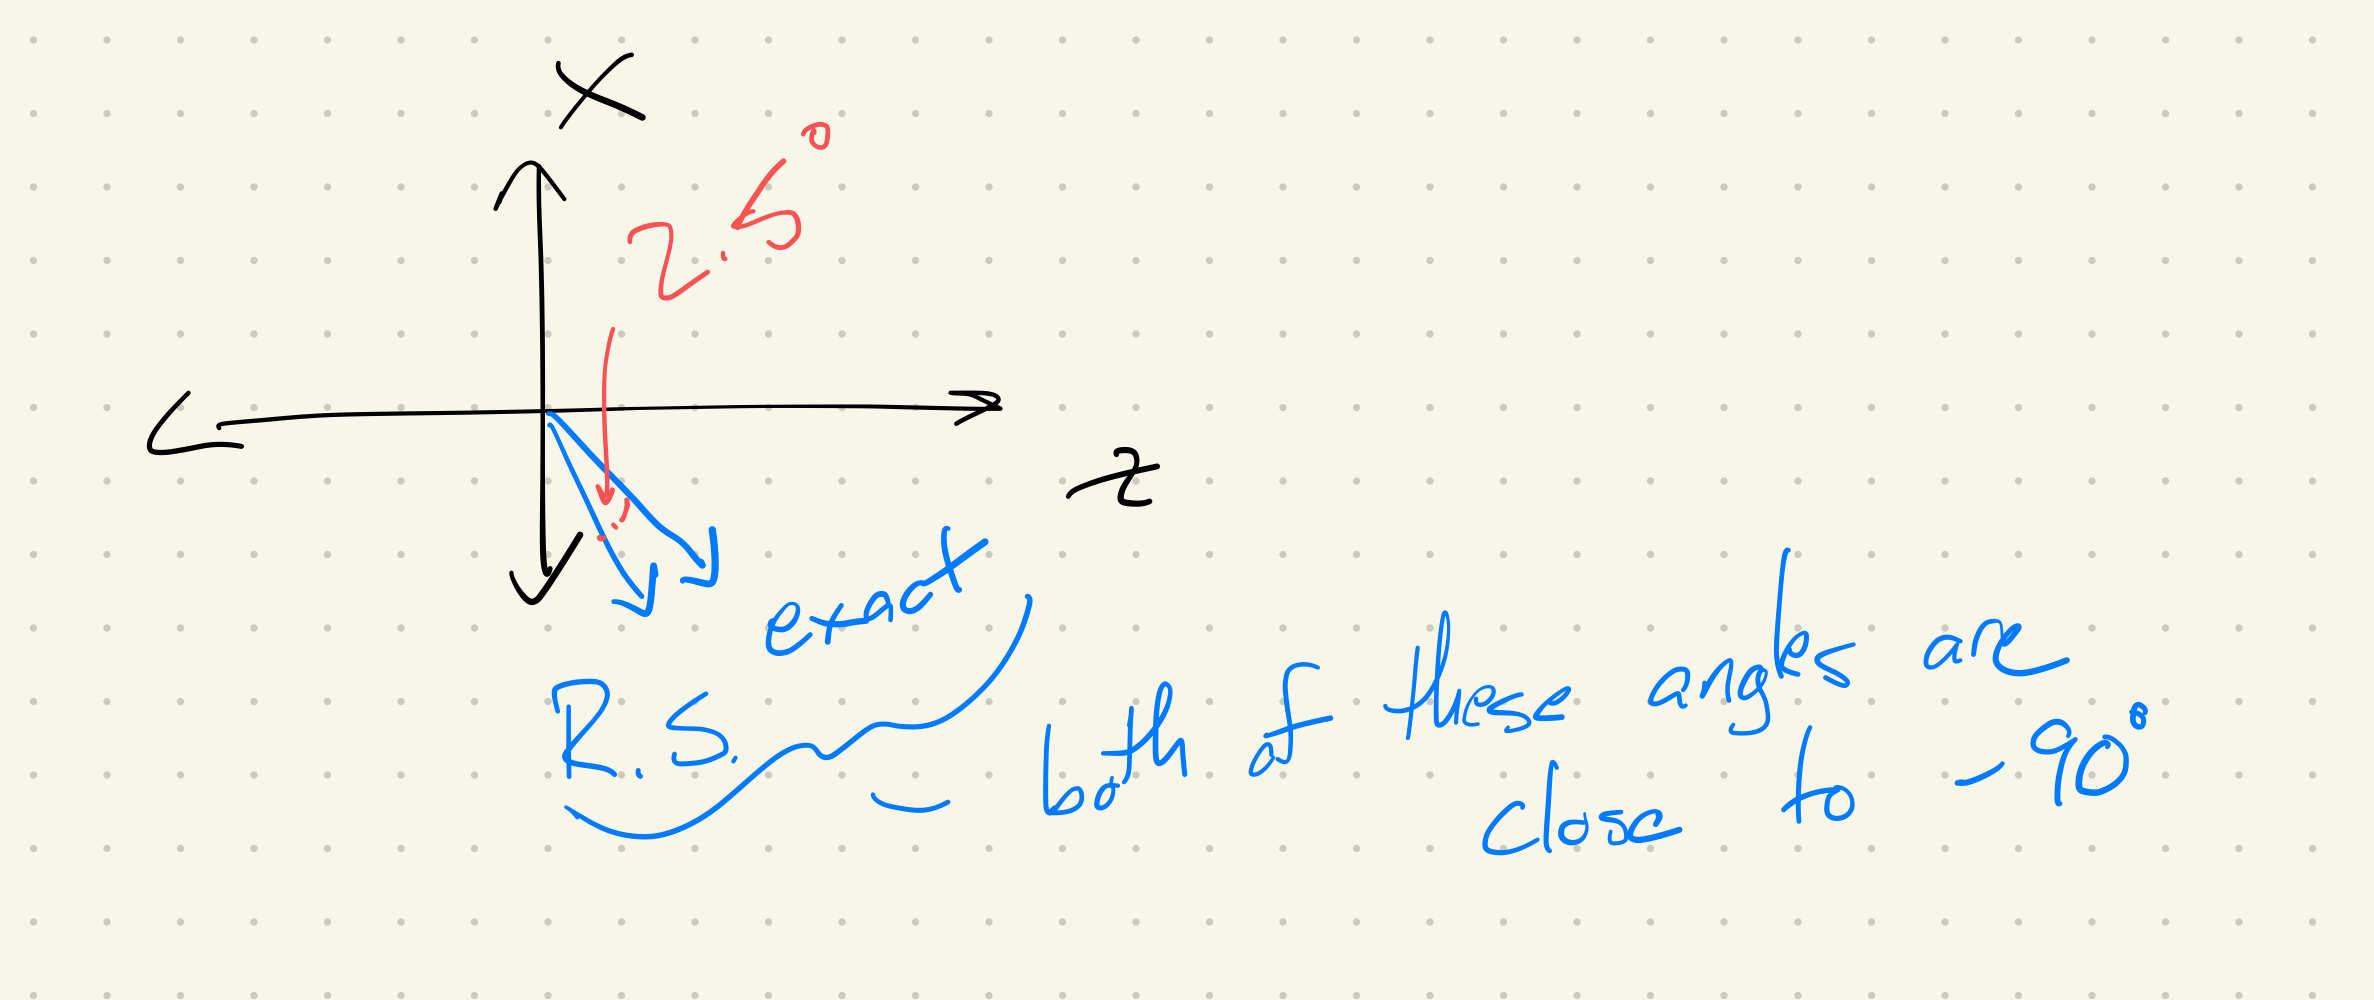
\includegraphics[width=.75\textwidth]{orient-sketch}
  \caption{Sketch of the approximate and exact orientation vectors}
  \label{fig:orient-sketch}
\end{figure}
  
% {\Large \textbf{Rolling tests with an ellipsoid in an unbounded shear
%     flow, and near a wall}}

% \begin{itemize}
% \item As an extension from the previous experiments with a sphere
%   rolling near a plane wall, I next ran experiments with an ellipsoid
%   with a minor axis of length $b = 0.5$, and major axes with length $a
%   = 1.5$.
% \item I ran tests with the ellipsoid in free space with three different
%   initial configurations, and two different mesh widths. The coarse
%   mesh had 386 Stokeslets on the platelet surface, and the fine mesh
%   width had 1538 Stokeslets. These two meshes had approximate widths
%   of $0.18$ and $0.09$ respectively.
% \item There are analytic solutions for the motion of an ellipsoid in
%   an unbounded shear flow, I used the expressions given in
%   \cite{Kim86}, which give the angular velocities as a function of the
%   ellipsoid orientation. Then I numerically integrated the ODE
%   $\frac{d\vect{e}_m}{dt} = \vect{\Omega} \times \vect{e}_m$ to get the
%   ``exact'' solution for the orientation of the platelet as a function
%   of time.
% \item Using the formulas from \cite{Kim86}, I also compared the
%   approximate angular velocities found by the regularized Stokeslets
%   method with the exact angular velocities at each time step, and
%   plotted the results.
% \item Plots of the orientation vector components, the error in
%   orientation as a function of time, and the error in the velocity
%   estimate at each step are plotted in Figures
%   \ref{fig:first-free-test}, \ref{fig:second-free-test}, and
%   \ref{fig:third-free-test}.
% \item In all three of these simulations, the orientation vector (the
%   minor axis) rotates around the $y$-axis. These are the Jeffery
%   orbits from \cite{Jeffery22}.
% \item The errors are largest in Figure \ref{fig:first-free-test},
%   where the orientation vector starts at $\vect{e}_x$, and is always
%   in the $x$--$z$ plane. The errors in the orientation get quite large
%   ($\sim 20\%$ for the coarse mesh, and $\sim 10\%$ for the fine
%   mesh), however this only occurs briefly--where the angular
%   velocities are the largest--and then the errors return to about 1/4
%   of their maximum point once the platelet has fully flipped over.
% \item Similar to the experiments with a sphere rolling near a wall,
%   the regularized Stokeslets method \emph{over}estimates the angular
%   velocity when the ellipsoid is ``flat'' in the shear flow ($\omega_y
%   < 0$, so the negative error shown in the plots corresponds to an
%   overestimate of the magnitude of the angular velocity). However,
%   when the minor axis is pointing in the direction of flow (the
%   platelet is ``vertical'' in the shear flow), the regularized
%   Stokeslets underestimate the angular velocity.
% \item When the orientation vector starts at $(1/\sqrt{2}, 1/\sqrt{2},
%   0)$, the errors are more than 2$\times$ smaller than the previous
%   case. There isn't much else to point out here, except that the
%   accuracy again improves by a factor of roughly 2 when the mesh width
%   is decreased.
% \item In the third free experiment, the orientation is initialized to
%   $\vect{e}_m = \vect{e}_y$. Here the orientation of the ellipsoid
%   remains constant, and there is some kind of symmetry that results in
%   errors canceling, and regularized Stokeslets accurately find the
%   angular velocities within machine precision (Figure
%   \ref{fig:third-free-test}). 
% \item In the three remaining figures, I show errors from experiments
%   where the ellipsoid was placed near a plane wall (all with an
%   initial orientation $\vect{e}_m = \vect{e}_x$). The center of the
%   ellipsoid was placed at initial heights of $1.5$, $1.2$, and $1.0$
%   in Figures \ref{fig:first-wall-test}, \ref{fig:second-wall-test},
%   and \ref{fig:third-wall-test} respectively.
% \item In these experiments, ``exact'' solutions were found by using an
%   even finer mesh ($\sim 1/3$ the width of the coarse mesh). The
%   ``exact'' simulations took $\sim 4.5$ hours to run on a single core
%   for 200 time steps. This means each time step takes about 80 sec.
% \item In Figure \ref{fig:first-wall-test}, we can nearly see a full
%   flip, and the shape of the orientation error is similar to the
%   unbounded case. That is, the coarse mesh overestimates the angular
%   velocity when the platelet is flat, and underestimates it when the
%   platelet is vertical.
% \item In the center of mass plot, we can see that the height of the
%   platelet increases slightly when the platelet is vertical. This has
%   to happen in order to give the platelet room to flip over.
% \item In the other two experiments, we don't get a full flip. I will
%   need to run a longer simulation in order to see that.
% \item I am also going to work on implementing receptor binding this
%   week. I'm thinking of tracking every receptor on the cell surface,
%   instead of the hybrid method I used for the 2D model. 
% \end{itemize}

% \begin{figure}
%   \centering
%   \begin{subfigure}{0.49\textwidth}
%     \includegraphics[width=\textwidth]{orient_plot11}
%   \end{subfigure}
%   \hfill
%   \begin{subfigure}{0.49\textwidth}
%     \includegraphics[width=\textwidth]{orient_plot16}
%   \end{subfigure}
%   \\
%   \begin{subfigure}{0.49\textwidth}
%     \includegraphics[width=\textwidth]{orient_err_plot11}
%   \end{subfigure}
%   \hfill
%   \begin{subfigure}{0.49\textwidth}
%     \includegraphics[width=\textwidth]{orient_err_plot16}
%   \end{subfigure}
%   \\
%   \begin{subfigure}{0.49\textwidth}
%     \includegraphics[width=\textwidth]{vel_err_plot11}
%   \end{subfigure}
%   \hfill
%   \begin{subfigure}{0.49\textwidth}
%     \includegraphics[width=\textwidth]{vel_err_plot16}
%   \end{subfigure}
%   \caption{Plots of the ellipsoid orientation, orientation error, and
%     velocity error in an unbounded shear flow. Orientation is
%     initialized at $\vect{e}_m = \vect{e}_x$. The three plots in the
%     left column are with the coarse mesh, and the three plots in the
%     right column are with the fine mesh. I didn't plot the center of
%     mass, because it remains constant.}
%   \label{fig:first-free-test}
% \end{figure}

% \begin{figure}
%   \centering
%   \begin{subfigure}{0.49\textwidth}
%     \includegraphics[width=\textwidth]{orient_plot21}
%   \end{subfigure}
%   \hfill
%   \begin{subfigure}{0.49\textwidth}
%     \includegraphics[width=\textwidth]{orient_plot26}
%   \end{subfigure}
%   \\
%   \begin{subfigure}{0.49\textwidth}
%     \includegraphics[width=\textwidth]{orient_err_plot21}
%   \end{subfigure}
%   \hfill
%   \begin{subfigure}{0.49\textwidth}
%     \includegraphics[width=\textwidth]{orient_err_plot26}
%   \end{subfigure}
%   \\
%   \begin{subfigure}{0.49\textwidth}
%     \includegraphics[width=\textwidth]{vel_err_plot21}
%   \end{subfigure}
%   \hfill
%   \begin{subfigure}{0.49\textwidth}
%     \includegraphics[width=\textwidth]{vel_err_plot26}
%   \end{subfigure}
%   \caption{Plots of the ellipsoid orientation, orientation error, and
%     velocity error in an unbounded shear flow. Orientation is
%     initialized at $\vect{e}_m = (1/\sqrt{2}, 1/\sqrt{2}, 0)^T$.}
%   \label{fig:second-free-test}
% \end{figure}

% \begin{figure}
%   \centering
%   \begin{subfigure}{0.49\textwidth}
%     \includegraphics[width=\textwidth]{orient_plot31}
%   \end{subfigure}
%   \hfill
%   \begin{subfigure}{0.49\textwidth}
%     \includegraphics[width=\textwidth]{orient_plot36}
%   \end{subfigure}
%   \\
%   \begin{subfigure}{0.49\textwidth}
%     \includegraphics[width=\textwidth]{orient_err_plot31}
%   \end{subfigure}
%   \hfill
%   \begin{subfigure}{0.49\textwidth}
%     \includegraphics[width=\textwidth]{orient_err_plot36}
%   \end{subfigure}
%   \\
%   \begin{subfigure}{0.49\textwidth}
%     \includegraphics[width=\textwidth]{vel_err_plot31}
%   \end{subfigure}
%   \hfill
%   \begin{subfigure}{0.49\textwidth}
%     \includegraphics[width=\textwidth]{vel_err_plot36}
%   \end{subfigure}
%   \caption{Plots of the ellipsoid orientation, orientation error, and
%     velocity error in an unbounded shear flow. Orientation is
%     initialized at $\vect{e}_m = \vect{e}_y$.}
%   \label{fig:third-free-test}
% \end{figure}

% \begin{figure}
%   \centering
%   \begin{subfigure}{0.49\textwidth}
%     \includegraphics[width=\textwidth]{orient_plot12}
%   \end{subfigure}
%   \hfill
%   \begin{subfigure}{0.49\textwidth}
%     \includegraphics[width=\textwidth]{orient_plot17}
%   \end{subfigure}
%   \\
%   \begin{subfigure}{0.49\textwidth}
%     \includegraphics[width=\textwidth]{orient_err_plot12}
%   \end{subfigure}
%   \hfill
%   \begin{subfigure}{0.49\textwidth}
%     \includegraphics[width=\textwidth]{orient_err_plot17}
%   \end{subfigure}
%   \\
%   \begin{subfigure}{0.49\textwidth}
%     \includegraphics[width=\textwidth]{com_plot12}
%   \end{subfigure}
%   \hfill
%   \begin{subfigure}{0.49\textwidth}
%     \includegraphics[width=\textwidth]{com_plot17}
%   \end{subfigure}
%   \caption{Plots of the ellipsoid orientation, orientation error, and
%     center of mass in a shear flow near a wall. The height of the
%     center of mass is initialized at $1.5$. Orientation is initialized
%     at $\vect{e}_m = \vect{e}_x$. The three plots in the left column
%     are with the coarse mesh, and the three plots in the right column
%     are with the fine mesh.}
%   \label{fig:first-wall-test}
% \end{figure}

% \begin{figure}
%   \centering
%   \begin{subfigure}{0.49\textwidth}
%     \includegraphics[width=\textwidth]{orient_plot13}
%   \end{subfigure}
%   \hfill
%   \begin{subfigure}{0.49\textwidth}
%     \includegraphics[width=\textwidth]{orient_plot18}
%   \end{subfigure}
%   \\
%   \begin{subfigure}{0.49\textwidth}
%     \includegraphics[width=\textwidth]{orient_err_plot13}
%   \end{subfigure}
%   \hfill
%   \begin{subfigure}{0.49\textwidth}
%     \includegraphics[width=\textwidth]{orient_err_plot18}
%   \end{subfigure}
%   \\
%   \begin{subfigure}{0.49\textwidth}
%     \includegraphics[width=\textwidth]{com_plot13}
%   \end{subfigure}
%   \hfill
%   \begin{subfigure}{0.49\textwidth}
%     \includegraphics[width=\textwidth]{com_plot18}
%   \end{subfigure}
%   \caption{Plots of the ellipsoid orientation, orientation error, and
%     center of mass in a shear flow near a wall. The height of the
%     center of mass is initialized at $1.2$. Orientation is initialized
%     at $\vect{e}_m = \vect{e}_x$. The three plots in the left column
%     are with the coarse mesh, and the three plots in the right column
%     are with the fine mesh.}
%   \label{fig:second-wall-test}
% \end{figure}

% \begin{figure}
%   \centering
%   \begin{subfigure}{0.49\textwidth}
%     \includegraphics[width=\textwidth]{orient_plot14}
%   \end{subfigure}
%   \hfill
%   \begin{subfigure}{0.49\textwidth}
%     \includegraphics[width=\textwidth]{orient_plot19}
%   \end{subfigure}
%   \\
%   \begin{subfigure}{0.49\textwidth}
%     \includegraphics[width=\textwidth]{orient_err_plot14}
%   \end{subfigure}
%   \hfill
%   \begin{subfigure}{0.49\textwidth}
%     \includegraphics[width=\textwidth]{orient_err_plot19}
%   \end{subfigure}
%   \\
%   \begin{subfigure}{0.49\textwidth}
%     \includegraphics[width=\textwidth]{com_plot14}
%   \end{subfigure}
%   \hfill
%   \begin{subfigure}{0.49\textwidth}
%     \includegraphics[width=\textwidth]{com_plot19}
%   \end{subfigure}
%   \caption{Plots of the ellipsoid orientation, orientation error, and
%     center of mass in a shear flow near a wall. The height of the
%     center of mass is initialized at $1.0$. Orientation is initialized
%     at $\vect{e}_m = \vect{e}_x$. The three plots in the left column
%     are with the coarse mesh, and the three plots in the right column
%     are with the fine mesh.}
%   \label{fig:third-wall-test}
% \end{figure}

\bibliographystyle{plain}
\bibliography{/Users/andrewwork/Documents/grad-school/thesis/library}

\end{document}




